% === [ Design ] ===============================================================

% <howto>
% * Justify, evaluate, recognize limitations of.
%
% * Analytical writing
%    - Why did you do X that way?
%    - Why did you do Y but not Z?
%    - What was important and what not?

\begin{quote}
	\textit{``The whole is more than the sum of its parts.''} - Anonymous
\end{quote}

\section{Design}
\label{sec:design}

The principle of separation of concern has had a core influence on the design of the decompilation system. It has motivated a system architecture which resembles a pipeline composed of independent components, each with access to the least amount of information required to successfully accomplish its task. Furthermore, a data-driven design separates data from source code to facilitate the extensibility of components.

Several smaller components may conceptually be arranged in a pipeline of stages which transform, massage or interpret the input in a certain way to solve larger tasks. A well composed pipeline is capable of solving more complex problems than each of its components, problems which may not even have been envisioned by the original component authors \cite{simplicity_and_collaboration}. This idea is embodied in the Unix philosophy and it has influenced software construction profoundly \cite{art_of_unix}. Furthermore, systems which expose their individual components to end-users facilitate dynamic workflows, as they enable users to adapt and extend each part of the system by adding, removing, replacing or refining components in one or more stages of the pipeline.

% TODO: <note> remove?
% Each component is self-contained any may be replated or used individually. It is possible to start with any component and use existing tools to bridge the gaps. <<< MOTIVATION: several starting points for a complex problem.

% TODO: Add design notes
%    - The LLVM IR libraries are developed as reusable components for compilers, decompilers, and other semantic analysis tools. They aim to support generic semantic analysis applications, while satisfying the explicit requirements [1] of the third party llgo compiler.
%
% [1]: https://github.com/go-llvm/llvm/issues/40

% TODO: Add
%   - The system must be language-agnostic so that decompilation passes can be reused from other programming language environments.

% --- [ System Architecture ] --------------------------------------------------

% <howto>
% * the overall structure of the software system (architecture)

% <howto>
% * Software architecture is concerned with deciding what has to be done, and which program component is going to do it (how something is done is left to the detailed design phase, below)
% * It effectively defines the interface between the programs of the system.
% * This stage does not need to consider non-functional requirements (e.g. response time, reliability, maintainability).

\subsection{System Architecture}

% TODO: Describe where the "restructure" component fits in the overall decompilation pipeline. Mention which projects and tools that may be used to fill the gaps. bin_descend and IDA python script of MC-Semantics -> Google Protocol Buffer -> cfg_to_bc -> LLVM IR

The decompilation pipeline conceptually consists of three modules which separate the major decompilation tasks (e.g. control flow analysis) from concerns related to the source or target language. Firstly, the front-end translates a variety of inputs (e.g. x86 or ARM assembly, Haskell or Rust source code, …) to LLVM IR by utilizing several independent open source projects. Secondly, the middle-end structures the LLVM IR by locating high-level control flow primitives. Lastly, the back-end translates the structured LLVM IR to a high-level target programming language (e.g. Go). The interaction between the front-end, middle-end and back-end modules is visualized in figure \ref{fig:decompilation_pipeline}.

% TODO: Find and add ref for \cite{llvm_architecture} and \cite{gcc_architecture}.

The main benefit with this decompiler architecture is that it scales well when adding support for new source languages (e.g. MIPS or PowerPC assembly) or target languages (e.g. Python), as the major decompilation tasks only have to be implemented once. The decompiler architecture is an adaptation of the one presented by C. Cifuentes back in 1994 (as described in section \ref{sec:decompilation_phases}), which was heavily inspired by the architecture of compilers that separated major optimization tasks (e.g. constant propagation) from concerns related to the source programming language (e.g. C) or target computer architecture (e.g. x86). The compiler architecture has been proven so effective at separating concerns that it remains in use by several production-quality compilers. %\cite{llvm_architecture,gcc_architecture}.

% * Front-end
%    - binary -> LLVM IR ([MC-Semantics](https://github.com/trailofbits/mcsema), [Dagger](http://dagger.repzret.org/) or [Fracture](https://github.com/draperlaboratory/fracture))
%    - source code -> LLVM IR (clang, ghc, rustc, ...)
% * Middle-end
%    - LLVM IR -> Unstructured CFG ([ll2dot](http://decomp.org/x/cmd/ll2dot))
%    - Unstructured CFG -> Structured CFG ([restructure](http://decomp.org/x/graphs/cmd/restructure).)
%       + Truthfully `ll2go` doesn't make direct use of `restructure` but rather the graph libraries.
% * Back-end
%    - Structured CFG -> Go ([ll2go](http://decomp.org/x/cmd/ll2go))
%    - Unpolished -> Go ([go-post](http://decomp.org/x/cmd/go-post))

\begin{figure}[htbp]
	\begin{center}
		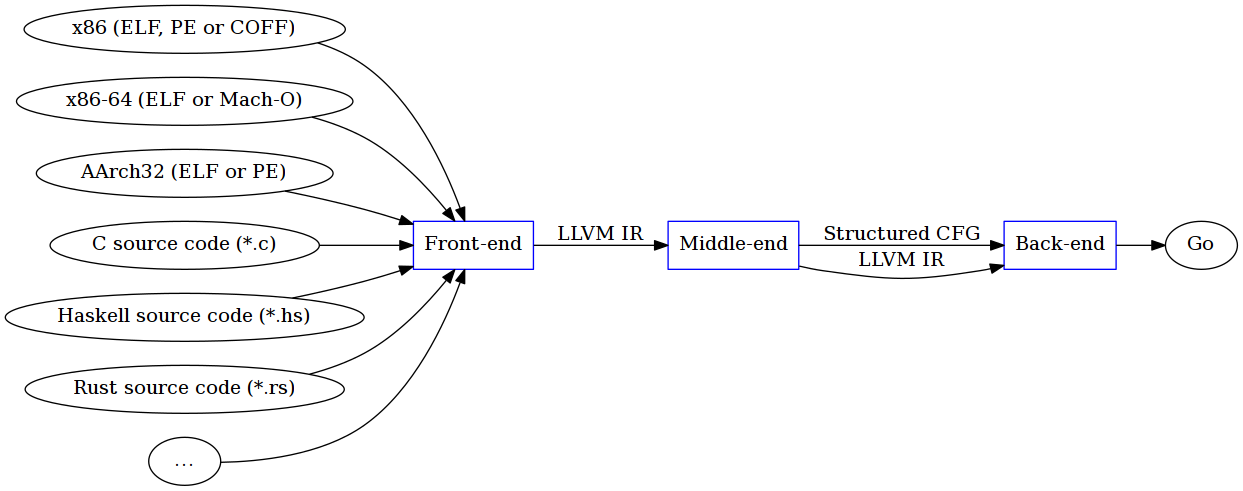
\includegraphics[width=\textwidth]{inc/decompilation_pipeline.png}
		\caption{The decompilation pipeline conceptually consists of three modules. Firstly, the front-end module translates native code to LLVM IR. Secondly, the middle-end structures the LLVM IR through control flow analysis. Lastly, the back-end translates the structured LLVM IR to the high-level programming language Go.}
		\label{fig:decompilation_pipeline}
	\end{center}
\end{figure}


\subsubsection{Front-end}

% TODO: Rewrite and clarify.

\textbf{NOTE}: \textit{The following paragraph is more of a brain-dump. It is intended to be used as a basis for a future rewrite.}

The front-end module is responsible for converting the input into LLVM IR. Two common scenarios exists, converting binary files (e.g. executables, shared libraries and relocatable object code) and converting source code (e.g. C, Haskell, Rust, …) into LLVM IR. The first scenario is presented in figure \ref{fig:front-end_binary} and the second in figure \ref{fig:front-end_source}.

% TODO: Mention opt --mem2reg.

\begin{figure}[htbp]
	\begin{center}
		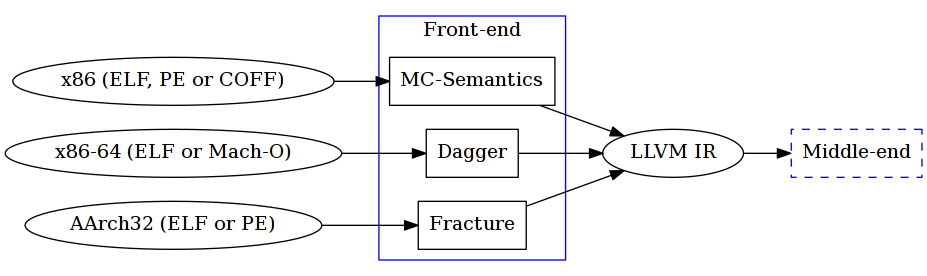
\includegraphics[width=\textwidth]{inc/front-end_binary.png}
		\caption{The three open source projects MC-Semantics, Dagger and Fracture translate native code of various architectures (e.g. x86, x86-64 and ARM) and file formats (e.g. ELF, PE, COFF and Mach-o) to LLVM IR.}
		\label{fig:front-end_binary}
	\end{center}
\end{figure}

\begin{figure}[htbp]
	\begin{center}
		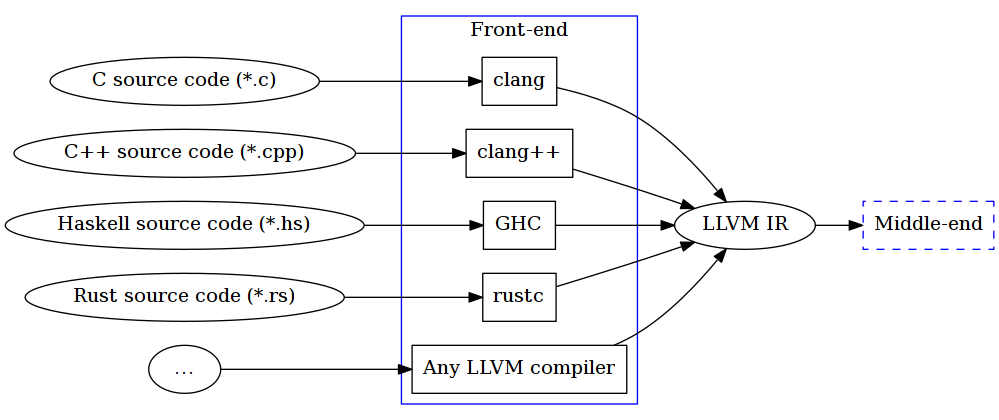
\includegraphics[width=\textwidth]{inc/front-end_source.png}
		\caption{Several open source compilers translate high-level programming languages to LLVM IR. Three such compilers are Clang, the Glasgow Haskell Compiler and the Rust compiler which translate C, Haskell and Rust respectively to LLVM IR.}
		\label{fig:front-end_source}
	\end{center}
\end{figure}

\subsubsection{Middle-end}

% TODO: Rewrite and clarify.

\textbf{NOTE}: \textit{The following paragraph is more of a brain-dump. It is intended to be used as a basis for a future rewrite.}

The middle-end is responsible for lifting the LLVM IR to a high-level representation through a series of decompilation passes. The \texttt{ll2dot} tool generates a CFG (in the DOT file format) for each function of a given LLVM IR input file. The \texttt{restructure} tool searches for subgraph isomorphisms of control flow primitives in a given CFG. Once located the nodes identified subgraph are merged into a single node which is labeled with the high-level control flow primitive. Successive iterations continue to simplify the CFG until only one node is left, at which point the high-level control flow structure has been recovered. Should the \texttt{restructure} tool fail to reduce the graph into a single node, the graph is considered irreducible with regards to the supported high-level control flow primitives. The interaction between the front-end, the \texttt{ll2dot} and \texttt{restructure} tools of the middle-end and the back-end is illustrated in figure \ref{fig:middle-end}.

% TODO: Write about the choice of subgraph isomorphism search algorithm. The
% properties of the control flow graph allows us to optimize.
%
% \cite{subgraph_isomorphism_algorithms}

\begin{figure}[htbp]
	\begin{center}
		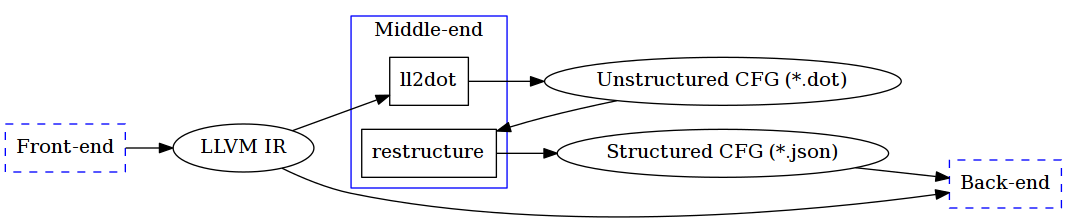
\includegraphics[width=\textwidth]{inc/middle-end.png}
		\caption{foo}
		\label{fig:middle-end}
	\end{center}
\end{figure}

\subsubsection{Back-end}

% TODO: Rewrite and clarify.

% TODO: Add ref to rsc's grind tool.

% TODO: Proof-of-concept. Implement a back-end for another language and written in another language. This would stress test the language-agnostic aspects of the design, thus making sure that the heavy-lifting is done in the middle-end and not in ll2go.

\textbf{NOTE}: \textit{The following paragraph is more of a brain-dump. It is intended to be used as a basis for a future rewrite.}

The back-end generates high-level control flow primitives such as if-statements and for-loops based on the structured CFG. In addition it translates the individual instructions of the LLVM IR to expressions and statements of the target programming language (in this case Go).

The back-end is responsible for translating the structured control flow graph of the LLVM IR into a target programming language. The \texttt{ll2go} tool is a proof of concept back-end which produces unpolished Go source code. The polishing is done by separate tools which fixes potential compilation issues and makes the code more idiomatic. The interaction between the middle-end and the back-end is illustrated in figure \ref{fig:back-end}. Currently the \texttt{go-post} replaces return-statements in the \texttt{main} function with calls to \texttt{os.Exit}, which is required since the \texttt{main} function has no return arguments in Go. Instead the Go runtime calls \texttt{os.Exit} with the status-code \texttt{0} once \texttt{main} returns to signal successful termination. This eliminates the need to always end the \texttt{main} function with a \texttt{return 0;} statement as is common practise in C. A future ambition is to make use of and possibly contribute to the \texttt{grind} tool which moves variable declarations closer to their usage, and thus improving readability of the code. Generally the aim is to keep the \texttt{ll2go} tool as simple as possible. The middle-end is responsible for the structural analysis, and as a future ambition the data flow analysis. Since the complexity of the back-end is kept to a minimum it should be trivial to implement support for other output languages.

\begin{figure}[htbp]
	\begin{center}
		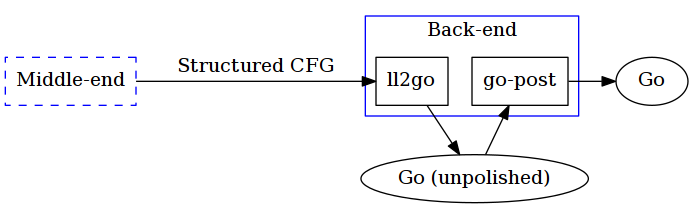
\includegraphics[width=\textwidth]{inc/back-end.png}
		\caption{foo}
		\label{fig:back-end}
	\end{center}
\end{figure}

% --- [ Front-end Components ] -------------------------------------------------

\subsection{Front-end Components}

foo

% ~~~ [ Native Code to LLVM IR ] ~~~~~~~~~~~~~~~~~~~~~~~~~~~~~~~~~~~~~~~~~~~~~~~

\subsubsection{Native Code to LLVM IR}

foo

% ~~~ [ Compilers ] ~~~~~~~~~~~~~~~~~~~~~~~~~~~~~~~~~~~~~~~~~~~~~~~~~~~~~~~~~~~~

\subsubsection{Compilers}

foo

% --- [ Middle-end Components ] ------------------------------------------------

% <howto>
% * more detailed design of individual components (design)

% <howto>
% * The intention is that the design should be detailed enough to provide a good guide for actual coding, including details of any particular algorithms to be used.

\subsection{Middle-end Components}

% TODO: Visualize the dependency graph of the "restructure" tool and describe in detail what input it expects and what output it produces.

% TODO: Write about. Input and output LLVM IR to operate well with components written in other languages. Output LLVM IR with information about high-level control structures stored in the basic block names or in metadata.

% TODO: Mention package division.

foo

% ~~~ [ Control Flow Graph Generation ] ~~~~~~~~~~~~~~~~~~~~~~~~~~~~~~~~~~~~~~~~

\subsubsection{Control Flow Graph Generation}

foo

% ~~~ [ Control Flow Analysis ] ~~~~~~~~~~~~~~~~~~~~~~~~~~~~~~~~~~~~~~~~~~~~~~~~

\subsubsection{Control Flow Analysis}

% TODO: Add
% * Subgraph Isomorphism Search Algorithm}

% * Data-driven Design (potential and limitations)
% TODO: Mention: CFG invariants (e.g. single-entry, single-exit)
% TODO: Add notes about the use of DOT-files to describe control flow primitives. Think if and how this could be pushed further to facilitate the development of future back-ends.

% TODO: Add: Limitations

% TODO: Add limitations related to the design choices. Which limitations are easily solvable given more time and which are fundamentally part of the design.
%    - No support for n-way conditionals (e.g.switch-statements).

foo

% --- [ Back-end Components ] --------------------------------------------------

\subsection{Back-end Components}

% ~~~ [ Code Generation ] ~~~~~~~~~~~~~~~~~~~~~~~~~~~~~~~~~~~~~~~~~~~~~~~~~~~~~~

\subsubsection{Code Generation}

foo

% ~~~ [ Post-processsing ] ~~~~~~~~~~~~~~~~~~~~~~~~~~~~~~~~~~~~~~~~~~~~~~~~~~~~~

\subsubsection{Post-processing}

foo
